\chapter{Analyse und Performance}

\section{Beurteilung der Anforderungserfüllung}

\section{Kostenaufstellung}
Die Kosten für die fertige Platine inklusive aller Bauteile belaufen sich bei einer einzigen Platine auf 80 Euro. Bei einer Stückzahl von 100 kann der Preis bereits auf 33,5 Euro gesenkt werden, während die Bauteilkosten bei einer Fertigung von 1000 Platinen nochmal auf knapp unter 25 Euro sinken. Diesen großen Preisunterschied verursacht vor allem die unbestückte Platine selbst, die bei Bestellung von einer einzigen 38,5 Euro kostet und bei einer Bestellung von 1000 Stück nur noch 0,82 Euro. Tabelle \ref{tab:Preisliste} zeigt die verwendeten Bauteile und deren Anzahl sowie den kumulierte Preis pro Bauteilart (Anzahl des Bauteils multipliziert mit dem Einzelpreis) für jeweils eine Fertigung von einer Platine, von 100 Platinen und von 1000 Platinen. Die Preise stammen dabei von den Anbietern, bei denen die Komponenten jeweils eingekauft wurden.

\begin{table}[h]
	\centering
\begin{tabular}{ | l | l | l | l | l | }
\hline
	Anzahl & Bauteil & Bauteilpreis & Bauteilpreis 100+ & Bauteilpreis 1000+\\ \hline
	1 & Platine & 38.5 Euro & 2.39 Euro & 0.82 Euro\\
	\  & \  & \  & \  & \  \\
	1 & Mikrocontroller & 10.66 Euro & 7.79 Euro & 6.58 Euro \\
	2 & Halbbrücken & 6.56 Euro & 5.96 Euro & 5.04 Euro\\
	1 & Leitungstreiber & 0.617 Euro & 0.348 Euro & 0.252 Euro \\
	1 & CAN Transceiver & 2.82 Euro & 2.28 Euro & 1.51 Euro \\
	1 & Voltage Regulator 3,3V & 0.337 Euro & 0.162 Euro & 0.103 Euro \\
	1 & Voltage Regulator 5V & 0.337 Euro & 0.162 Euro & 0.103 Euro \\
	\  & \  & \  & \  & \  \\
	1 & Klemmblock & 1.16 Euro & 1.07 Euro & 0.912 Euro \\
	2 & Klemmblock & 0.742 Euro & 0.618 Euro & 0.526 Euro \\
	1 & Steckverbinder & 0.0442 Euro & 0,0442 Euro & 0,0387 Euro \\
	1 & AMPSEAL Automotive Steckverbinder & 7.09 Euro & 6.22 Euro & 5.23 Euro\\
	\  & \  & \  & \  & \  \\
	1 & Quarz & 0.605 Euro & 0.355 Euro & 0.384 Euro \\
	21 & Widerstände & 4.88 Euro & 3.046 Euro & 1.6754 Euro\\
	21 & Kondensatoren & 5.907 Euro & 3.0648 Euro & 1.501 Euro\\ \hline
	\  & \textbf{Gesamtpreis} & \textbf{80,26 Euro}  & \textbf{33,51 Euro}  & \textbf{24,68 Euro}  \\ \hline
\end{tabular}
\caption{Preisliste}
	\label{tab:Preisliste}
\end{table}

Die gesamte Preisauflistung für die Stückzahlen eins, 100 und 1000 inklusive der einzelnen Widerstände und Kondensatoren, sowie die Händlerlinks zu allen Bauteilen befindet sich im Anhang.
In nachfolgenden Abbildungen wird die Verteilung der Kosten auf die verschiedenen Bauteilgruppen dargestellt. Die Bauteile wurden unterteilt in die Platine, die passiven Bauteile (Kondensatoren, Widerstände und Schwingquarz), die integrierten Halbleiterchips (Mikrocontroller, Spannungsregler, CAN Transceiver, Leitungstreiber, Halbbrücken) sowie die Stecker, die die Schnittstellen nach außen darstellen. 

\begin{figure}[h]
\begin{minipage}[h]{0.5\textwidth}
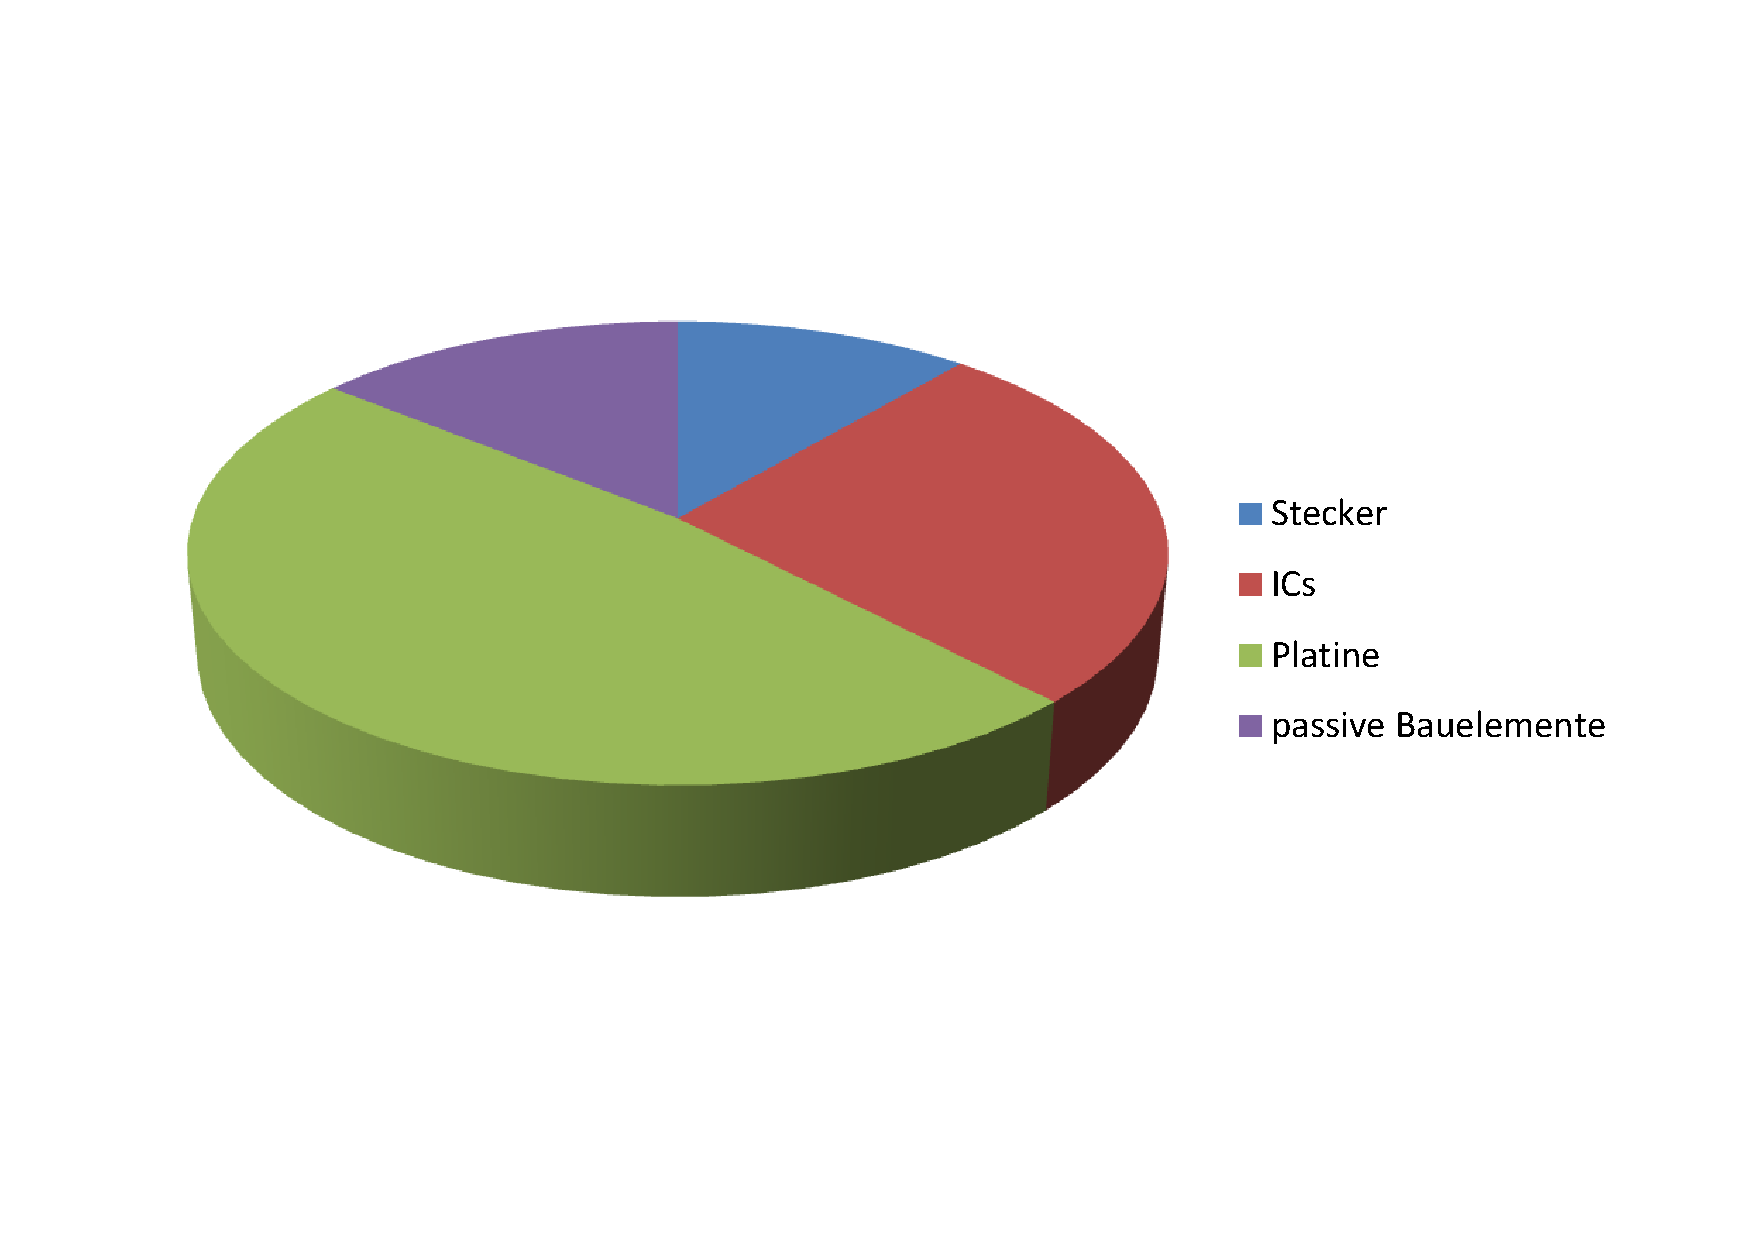
\includegraphics[width=\textwidth]{./Bilder/Platinenkosten.pdf}
\end{minipage}
\begin{minipage}[h]{0.5\textwidth}
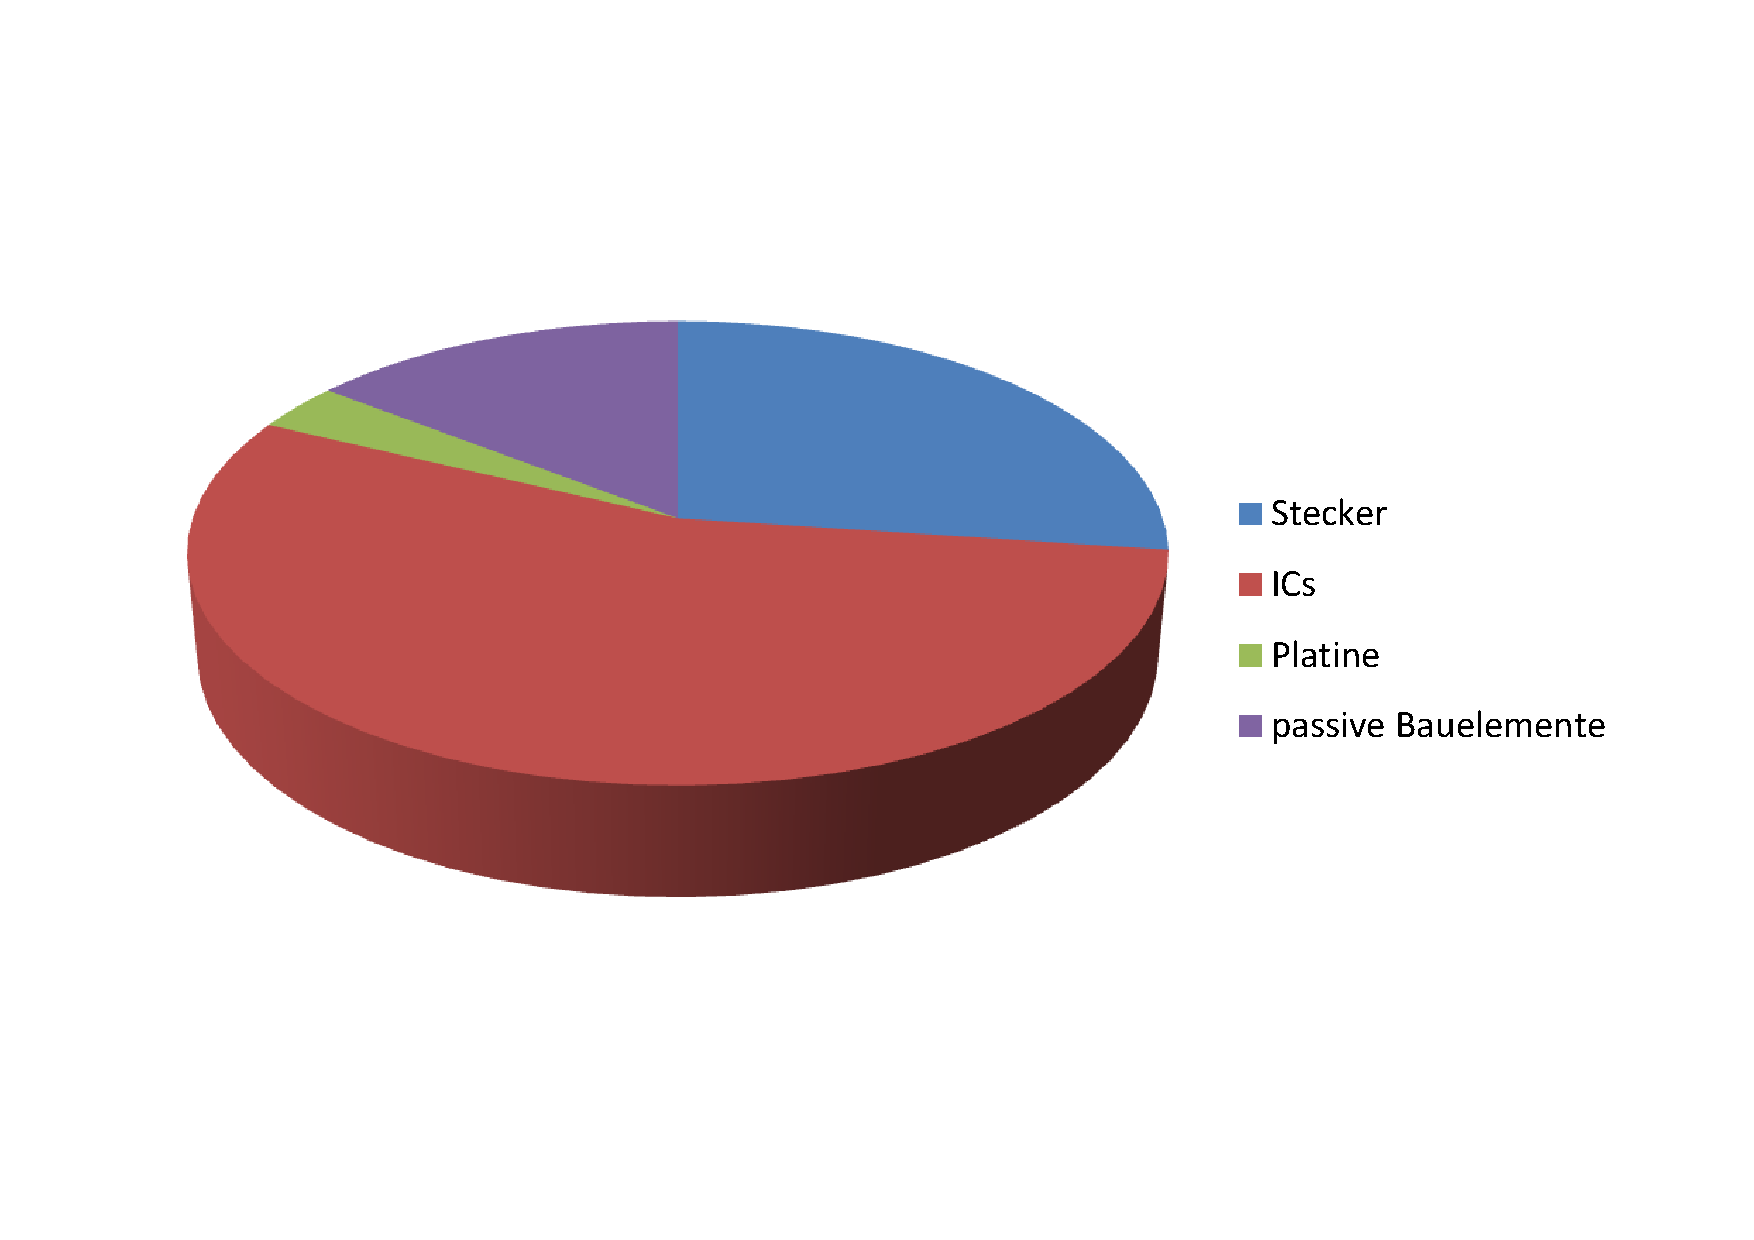
\includegraphics[width=\textwidth]{./Bilder/Platinenkosten-tausend.pdf}
\end{minipage}
\caption{Aufteilung der Kosten für die Stückzahlen 1 (links) und 1000 (rechts)}
	\label{fig:LDO}
\end{figure}

Es ist zu erkennen, dass bei geringen Stückzahlen die Platine ungefähr die Hälfte der Kosten ausmacht, während sie bei hohen Stückzahlen fast gar nicht mehr ins Gewicht fällt. Bei hohen Stückzahlen sind der größte Kostenfaktor die ICs. 


